\chapter{Protection}
\label{chap:constantTimeSolution}

Ce deuxième chapitre montre les innovations nécessaires pour se protéger des attaques temporelles. On y découvre les bonnes pratiques de programmation, les premiers outils automatique de vérification de code ainsi que les limitations auquelles est confronté le développeur qui souhaite être résistant à ces attaques.


\section{Bonne pratique et usages}

Face à la menace des attaques temporelles, quelles solutions peuvent être mises en place pour protéger nos systèmes informatiques ? Cette attaque a besoin d'un accès au système et d'un chronomètre. Comme on est dans un contexte de systèmes accessibles par internet, altérer ou retirer l'accès signifie perdre en qualité ou supprimer le service proposé. Il faut donc que notre approche cible plutôt l'utilisation du chronomètre.

Il faut donc programmer de tel sorte que sur toutes les entrées possibles de notre système informatique aucune variation de temps ne peut être observée entre les exécutions.
Trois méthodes existent pour pallier à ce problème.\medbreak

\subsection*{Programmation en temps constant}
La programmation en temps constant ou <<\textit{Constant-Time Programming}>>, est une pratique de programmation qui vise à résoudre exactement ce problème. Directement lié à la compléxité algorithmique, cette pratique modifie et adapte les algorithmes pour que toutes les opérations effectuées aient un temps d'exécution identique.

\citeauthor{BearSSL} \cite{BearSSL} présente tous les éléments à adapter pour configurer un code respectant la politique de programmation en temps constant. Si les opérations élémentaires respectent "naturellement" cette politique; les \textbf{accès mémoires}, les \textbf{sauts conditionnels}, les \textbf{sopérations de décalages/rotations} et les \textbf{divisions/multiplications} sont les opérations à adapter en fonction de la plateforme cible. Les descriptions rapportées ci-dessous sont issues de \cite{BearSSL}.\smallbreak

\begin{CitationBox}{Accès mémoire}
  Un chargement depuis la mémoire d'une information est une source de variation. On a vs précedemment \cite{LLC_attack,DRAM_Attack} que l'usage d'un cache mémoire est un canal d'accès pour réaliser une attaque. En effet, l'utilisation d'un cache permet de distinguer les appels entre les données déjà mises en mémoire ou pas. De plus, les changements de valeur dans celui-ci peuvent aussi être observé après exécution.
\end{CitationBox}
\vspace{0.1cm}
\begin{CitationBox}{Décalage et rotation}
  Ces opérations binaires sont ou ne sont pas en temps constant en fonction des CPU sur lequel le code est exécuté. Certains ont un "barrel shifter" qui permet d'effectuer directement les instructions correspondantes. Cela impacte directement les algorithmes dépendant de décalages logiques comme le chiffrement RC5.
\end{CitationBox}
\vspace{0.1cm}
\begin{CitationBox}{Saut conditionnel}
  Les saut conditionnels sont des instructions qui, comme pour les accès mémoires, demandent de charger les adresses des instructions suivantes. Or, comme un compilateur tend à précharger les instructions suivantes, il va charger les deux côtés du saut conditionnel puis defausser la branche inutile; ce qui entraîne un léger alentissement. En revanche, il est important de noter que si le branchement est indépendant d'une variable secrète, il n'est pas nécessaire de le modifier. Par exemple si j'ai un compteur et que mon programme doit terminer après un certain nombre d'itérations, aucune fuite ne sera observée.
\end{CitationBox}
\vspace{0.1cm}
\begin{CitationBox}{Division}
  Certaines architectures ont des instructions de divisions spécifiques qui permettent d'accélérer le calcul, les autres emploient des sous-programmes dédiées souvent optimisés en opération de masquage et de décalage. La norme C entraîne elle aussi de la confusion car elle impose $(-1)/2 = 0$; il faut donc être familier avec les spécificités du processeur pour affiner l'usage de cette opération.
\end{CitationBox}
\vspace{0.1cm}
\begin{CitationBox}{Multiplication}
  Enfin, la multiplication, elle aussi dépendante des variable d'entrées, présente une fuite d'information importante. Mais les CPU les plus récents (rédigé en 2016) ont implémenté cette opération en temps constant. Cela suit l'évolution des compilateurs et des processeurs qui tendent à accélérer les opérations et réduire le nombre d'instruction total.
\end{CitationBox}
\vspace{0.1cm}

En reprennant ces règles, on peut modifier notre exemple de code \ref{lst:timing_attack_example} et appliquer des modifications sur lignes que l'on a déjà ciblées comme fuites d'informations. Les modifications sont libre au choix du concepteur. Voici une correction qui peut être réalisée :

\begin{listing}[!htb]
    \caption{Exemple de correction pour rendre un code résistant aux attaques temporelles}
    \label{lst:timing_attack_CT_example}
    \begin{minted}[frame=lines,framesep=2mm,baselinestretch=1.2,fontsize=\footnotesize,linenos, gobble=6]{C}
        bool check_pwd(msg,pwd) {
          // Hachage
            char msg_hash[SHA256_DIGEST_LENGTH]; sha256_hash_string(msg, msg_hash);
            char pwd_hash[SHA256_DIGEST_LENGTH]; sha256_hash_string(pwd, pwd_hash);

            // Comparaison
            bool equal = true;
            for (int i = 0; i < SHA256_DIGEST_LENGTH; i++) {
                if (msg_hash[i] != pwd_hash[i]) {
                    equal = equal && false;
                } else {
                    equal = equal || false;
                }
            }
            return equal;
        }
    \end{minted}
\end{listing}

On voit que le premier branchement a été remplacé par un hachage des paramètres d'entrées. Cette opération est considérée ici en temps constant mais peut ne pas l'être. Il faut être vigilant sur toutes les briques d'algorithme que l'on souhaite utiliser. Enfin, le second branchement conditionnel est purement supprimé, le parcours des tableaux se fait entièrement.\bigbreak

Avec cette modification, on a un code \ref{lst:timing_attack_CT_example} qui ne présente plus de fuite de données. Pourtant, on peut avoir un doute sur l'usage de la fonction "\textit{sha256\_hash\_string}". Si cette fonction n'est pas elle même implémentée selon la politique temps constant, on a alors introduis une nouvelle surface de fuite d'informations. Il faut vérifier notre code pour supprimer ce doute.\medbreak

\subsection*{Outils de garanties}

Plusieurs outils existent est peuvent être utilisés tous au long du processus de développement d'un système sécurisé. Cela peut être durant la phase de conception du code source, au moment de la compilation ou encore en vérification de la compilation.\smallbreak


Une solution légère est de ce servir du système libre <<\textbf{Compiler Explorer}\footnote{\url{https://godbolt.org/}}>>. Avec à disposition un éditeur de texte, il est possible de voir comment sera généré le code assembleur. En reprenant une partie du code \ref{fig:timing_attack_example}, on peut voir sur la figure \ref{img:godbolt_example} que le choix du compilateur, ici sa version, introduit une légère modification. Ce changement n'est pas perceptible sans observation directe, il se perçoit directement grâce à la petite taille du code observé.

\begin{figure}[!h]
  \begin{adjustwidth}{-2.5cm}{-2cm}
    \centering
    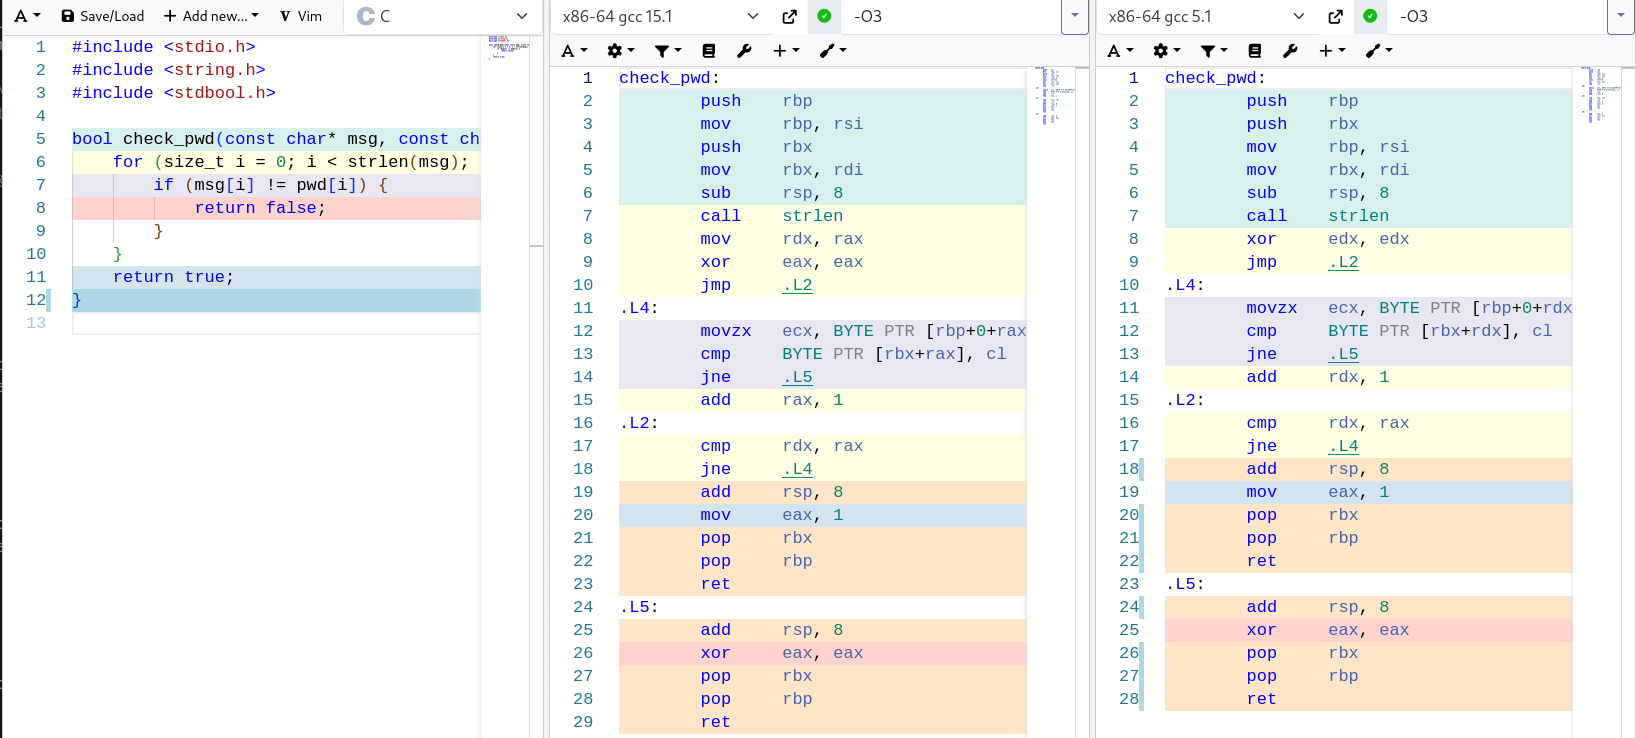
\includegraphics[trim = 1mm 0mm 0mm 0mm, clip,width=0.9\paperwidth]{pictures/godbolt_example.png}
    \caption{Capture d'écran de comparaison de code assembleur x86\_64 entre \texttt{GCC 15.1} et \texttt{GCC 5.1}}
    \label{img:godbolt_example}
  \end{adjustwidth}
\end{figure}

Si l'on souhaite faire une analyse à l'échelle d'un projet, ce parcours à la main des fonctions ou de morceaux de fonctions est réellement fastidieux. Il faut mieux déléguer ce travail à un outil conçus pour vérifier la présence de fuite.\smallbreak

Plusieurs articles références l'ensemble des outils existant \cite{notThatHardCT, GeimerEvaluationsSideChannel} pour réaliser ce travail. Le tableau \ref{tab:tools_ct} de \citeauthor{notThatHardCT} liste 24 outils en libre accès conçus pour détecter des failles par canal auxiliaire.

Ils sont listés alphabétiquement et sont précisé le type de fichier analysé (\textit{Cible}), la méthode d'analyse réalisée (\textit{Techn.}) et les garanties attendues de ces analyses (\textit{Garanties}). On reviendra plus en avant avec ces détails de méthodes et de fonctionnement dans le chapitre \ref{chap:automateVerifOutils}.\medbreak

\begin{table}[!ht]
  \caption{Liste d'outils de vérification, source \cite{notThatHardCT} }
  \label{tab:tools_ct}
  \scriptsize{
  Cible : [C, Java] = Code source, Binaire = Binaire, DSL = Surcouche de langage, Trace = Trace d'exécution, WASM = Assembleur web.\\
  Techn. : Formel = Programmation formelle, [Symbolique, Dynamique, Statistique] = type d'analyse. \\
  Garanties (\textit{Sécurité face aux attaques temporelles}) : $\bullet$ = Analyse correct, $\blacktriangle$ = Correct mais avec des limitations, $\circ$ = Aucune garantie, $\bigstar$ = Vérification d'autres propriétés.
  }
  \normalsize
  \begin{center}
    \begin{tabular}{lccc}
    \hlineB{2}
    \textbf{Outil} & \textbf{Cible} & \textbf{Techn.} & \textbf{Garanties} \\
    \rowcolor{lightgray}
    ABPV13 \cite{ABPV13} & C & Formel & $\bullet$ \\
    Binsec/Rel \cite{binsecRel2019} & Binaire & Symbolique & $\blacktriangle$ \\
    \rowcolor{lightgray}
    Blazer \cite{Blazer} & Java & Formel & $\bullet$ \\
    BPT17 \cite{BPT17} & C & Symbolique & $\blacktriangle$ \\
    \rowcolor{lightgray}
    CacheAudit \cite{CacheAudit} & Binaire & Formel & $\bigstar$ \\
    CacheD \cite{CacheD} & Trace & Symbolique & $\circ $ \\
    \rowcolor{lightgray}
    COCO-CHANNEL \cite{COCOCHANNEL} & Java & Symbolique & $\bullet$ \\
    ctgrind \cite{ctgrind} & Binaire & Dynamique & $\blacktriangle$ \\
    \rowcolor{lightgray}
    ct-fuzz \cite{ctfuzz} & LLVM & Dynamique & $\circ$ \\
    ct-verif \cite{ctverif} & LLVM & Formel & $\bullet$ \\
    \rowcolor{lightgray}
    CT-WASM \cite{CTWASM} & WASM & Formel & $\bullet$ \\
    DATA \cite{DATA1,DATA2} & Binaire & Dynamique & $\blacktriangle$ \\
    \rowcolor{lightgray}
    dudect \cite{dudect} & Binaire & Statistique & $\circ $ \\
    FaCT \cite{FaCT} & DSL & Formel & $\bullet$ \\
    \rowcolor{lightgray}
    FlowTracker \cite{FlowTracker} & LLVM & Formel & $\bullet$ \\
    haybale-pitchfork \cite{haybale-pitchfork} & LLVM & Symbolique & $\blacktriangle$ \\
    \rowcolor{lightgray}
    KMO12 \cite{KMO12} & Binaire & Formel & $\bigstar$ \\
    MemSan \cite{MemSan} & LLVM & Dynamique & $\blacktriangle$ \\
    \rowcolor{lightgray}
    MicroWalk \cite{MicroWalk} & Binaire & Dynamique & $\blacktriangle$ \\
    SC-Eliminator \cite{SCEliminator} & LLVM & Formel & $\bullet$ \\
    \rowcolor{lightgray}
    SideTrail \cite{SideTrail} & LLVM & Formel & $\bigstar$ \\
    Themis \cite{Themis} & Java & Formel & $\bullet$ \\
    \rowcolor{lightgray}
    timecop \cite{timecop} & Binaire & Dynamique & $\blacktriangle$ \\
    VirtualCert \cite{VirtualCert} & x86 & Formel & $\bullet$ \\
    \hlineB{2}
    \end{tabular}
  \end{center}
\end{table}

\newpage
Une dernière solution serait d'utiliser un compilateur spécialisé qui produit un code assembleur sans fuite \cite{Borrello_2021, Raccoon} ou d'utiliser un compilateur formel comme \textit{CompCert} \cite{CompCert}. Cette solution rencontre en pratique de nombreux problèmes que l'on se garde pour la section \ref{sect:limitations} \nameref{sect:limitations}.

\subsection*{Écriture en code assembleur}

Enfin, la dernière méthode pour obtenir un code sécurisé et sans fuite c'est de programmer directment en assembleur. De cette manière, on a un contrôle total sur le flot d'exécution de notre programme, on peut ainsi insérer des optimisations qu'un compilateur pourrait ignorer. Écrire en assembleur requiert de connaître la plupart des opérandes disponibles pour l'architecture que l'on cible et les modèles des composants présents sur le support. Cela nous amène directement aux limitations induites par cette solution.

\section{Limitations}
\label{sect:limitations}

Écrire en assembleur c'est écrire spécifiquement pour une architecture de processeur. Il faut connaître les instructions adéquates, les potentielles optimisations qui existent sans parler de la synthaxe particulère qui rend son développement plus lent. Travailler en assembleur c'est limiter la portabilité du code proposé. Or l'objectif derrière le développement d'une librairie sécurisée est de pouvoir être employée par le plus de configurations possibles pour se protéger d'attaques.\smallbreak

Face à cette situation, on choisit donc d'utiliser un compilateur spécialisé (\cite{Borrello_2021, Raccoon}). Et à nouveau on se retrouve limité parce que ces compilateurs ne supportent pas l'ensemble du jeu d'instruction d'une architecture, ont besoin d'instructions supplémentaires (des annotations de code) pour réaliser la compilation, n'implémente pas les optimisations qui apparaissent sur les processeurs les plus récents ou encore ne sont adaptés qu'à un seul langage de programmation.\smallbreak

À nouveau, on se retrouve donc à utiliser les compilateurs communs \texttt{GCC} et \texttt{LLVM} pour notre solution sécurisée. On se doit donc de programmer en respectant la politique temps constant. Et si cette pratique semble faire ses preuves, on peut lire dans la présentation de l'outil d'analyse Binsec \citetitle{binsecRel2019} : 
\begin{CitationBox}{Conclusion - \cite{binsecRel2019}}
Nous avons découvert que \texttt{gcc -O0} et des optimisations de \texttt{clang} introduisent des infractions à la politique temps constant indétectées par les outils antérieurs
\end{CitationBox}\smallbreak

Cette annonce a ensuite été prise en compte par \citeauthor{schneider2024breakingbadcompilersbreak} qui a mené une enquête sur les bibliothèques cryptographiques sécurisées et résistantes aux attaques temporelles : \cite{schneider2024breakingbadcompilersbreak}. La conclusion principale est que les compilateurs modernes sont devenus assez performants pour voir à travers les astuces employées et qu'une mauvaise utilisation d'optimisation implique l'introduction de faille de sécurité. \smallbreak

Voici un exemple communiqué par \citeauthor{schneider2024breakingbadcompilersbreak} auprès des chercheurs de Hacl*. On peut voir deux fonctions dans le code \ref{lst:Hacl_masking}, <<\textit{cmovznz4}>> et <<\textit{FStar\_UInt64\_eq\_mask}>>. La première appelle la seconde pour générer un masque qui sera ensuite appliqué au entrée de <<\textit{cmovznz4}>>. On a ici une fonction qui agit comme un branchement conditionnel. Si \texttt{cin} vaut 1, alors $r = x$ sinon $r = y$.

\begin{listing}[!ht]
    \caption{Fonction de masquage issu de \textit{Hacl*}}
    \label{lst:Hacl_masking}
    \begin{minted}[frame=lines,framesep=2mm,baselinestretch=1.2,fontsize=\footnotesize,linenos]{C}
#include <stdint.h>

static inline uint64_t FStar_UInt64_eq_mask(uint64_t a, uint64_t b)
{
  uint64_t x = a ^ b;
  uint64_t minus_x = ~x + (uint64_t)1U;
  uint64_t x_or_minus_x = x | minus_x;
  uint64_t xnx = x_or_minus_x >> (uint32_t)63U;
  return xnx - (uint64_t)1U;
}

void cmovznz4(uint64_t cin, uint64_t *x, uint64_t *y, uint64_t *r)
{
  uint64_t mask = ~FStar_UInt64_eq_mask(cin, (uint64_t)0U);
  uint64_t r0 = (y[0U] & mask) | (x[0U] & ~mask);
  uint64_t r1 = (y[1U] & mask) | (x[1U] & ~mask);
  uint64_t r2 = (y[2U] & mask) | (x[2U] & ~mask);
  uint64_t r3 = (y[3U] & mask) | (x[3U] & ~mask);
  r[0U] = r0;
  r[1U] = r1;
  r[2U] = r2;
  r[3U] = r3;
}
    \end{minted}
\end{listing}

Avec le compilateur \texttt{RISC-V rv64gc clang 15.0.0}, si on entre les options de compilation \texttt{-O0} ou \texttt{-O1} on peut observer différents résultats. Le plus notable ici est l'apparition de l'instruction \texttt{beqz}, qui est un branchement conditionnel, ainsi que la suppression de la fonction de masquage <<\textit{FStar\_UInt64\_eq\_mask}>>. Les optimisations appelées par l'option \texttt{-O1} identifient le masquage réalisé et modifient le code pour accélérer son exécution. L'optimisation \ref{subcode:O0} suient les instructions précisées par le code source, de cette manière le compilateur réalise une compilation rapide. Au contraire dde l'optimisation \ref{subcode:O1} qui réalise une analyse plus longue du code source, et donc a une compilation plus lente, mais grâce à l'ajout des branchements succesifs (les instructions \texttt{beqz}) permet une exécution plus rapide. Les options de compilations sont rapportées en annexe \ref{tab:compile_option}\footnote{\url{https://gcc.gnu.org/}}.

\begin{figure}[!ht]
    \begin{subfigure}[b]{0.5\textwidth}
        \centering
        \small
        \begin{minted}[frame=single, framesep=2mm, baselinestretch=1.2, fontsize=\footnotesize, linenos]{java}
cmovznz4:
        ...
        li      a1, 0
        call    FStar_UInt64_eq_mask
        not     a0, a0
        sd      a0, -56(s0)
        ld      a0, -40(s0)
        ld      a0, 0(a0)
        ld      a2, -56(s0)
        and     a0, a0, a2
        ld      a1, -32(s0)
        ld      a1, 0(a1)
        not     a2, a2
        and     a1, a1, a2
        or      a0, a0, a1
        sd      a0, -64(s0)
        ...
        ret

FStar_UInt64_eq_mask:
        addi    sp, sp, -64
        sd      ra, 56(sp)
        sd      s0, 48(sp)
        addi    s0, sp, 64
        sd      a0, -24(s0)
        sd      a1, -32(s0)
        ld      a0, -24(s0)
        ld      a1, -32(s0)
        xor     a0, a0, a1
        sd      a0, -40(s0)
        ld      a1, -40(s0)
        li      a0, 0
        sub     a0, a0, a1
        sd      a0, -48(s0)
        ld      a0, -40(s0)
        ld      a1, -48(s0)
        or      a0, a0, a1
        sd      a0, -56(s0)
        ld      a0, -56(s0)
        srli    a0, a0, 63
        sd      a0, -64(s0)
        ld      a0, -64(s0)
        addi    a0, a0, -1
        ld      ra, 56(sp)
        ld      s0, 48(sp)
        addi    sp, sp, 64
        ret
        \end{minted}
        \caption{Option \texttt{-O0}}
        \label{subcode:O0}
    \end{subfigure}%
    ~~
    \begin{subfigure}[b]{0.4\textwidth}
        \centering
        \small
        \begin{minted}[frame=single, framesep=2mm, baselinestretch=1.2, fontsize=\footnotesize, linenos]{java}
cmovznz4:
        mv      a5, a1
        beqz    a0, .LBB0_2
        mv      a5, a2
.LBB0_2:
        beqz    a0, .LBB0_5
        addi    a6, a2, 8
        bnez    a0, .LBB0_6
.LBB0_4:
        addi    a4, a1, 16
        j       .LBB0_7
.LBB0_5:
        addi    a6, a1, 8
        beqz    a0, .LBB0_4
.LBB0_6:
        addi    a4, a2, 16
.LBB0_7:
        ld      a7, 0(a5)
        ld      a5, 0(a6)
        ld      a6, 0(a4)
        beqz    a0, .LBB0_9
        addi    a0, a2, 24
        j       .LBB0_10
.LBB0_9:
        addi    a0, a1, 24
.LBB0_10:
        ld      a0, 0(a0)
        sd      a7, 0(a3)
        sd      a5, 8(a3)
        sd      a6, 16(a3)
        sd      a0, 24(a3)
        ret
        \end{minted}
        \caption{Option \texttt{-O1}}
        \label{subcode:O1}
    \end{subfigure}
    \caption{Comparaison du code \ref{lst:Hacl_masking} en fonction de différentes options de compilation données au compilateur, réalisée avec l'aide de \textit{Compiler Explorer}.}
\end{figure}

\raggedbottom
\textit{Transition}
